\documentclass{standalone}
\usepackage{tikz}
\usetikzlibrary{patterns, positioning}


\begin{document}
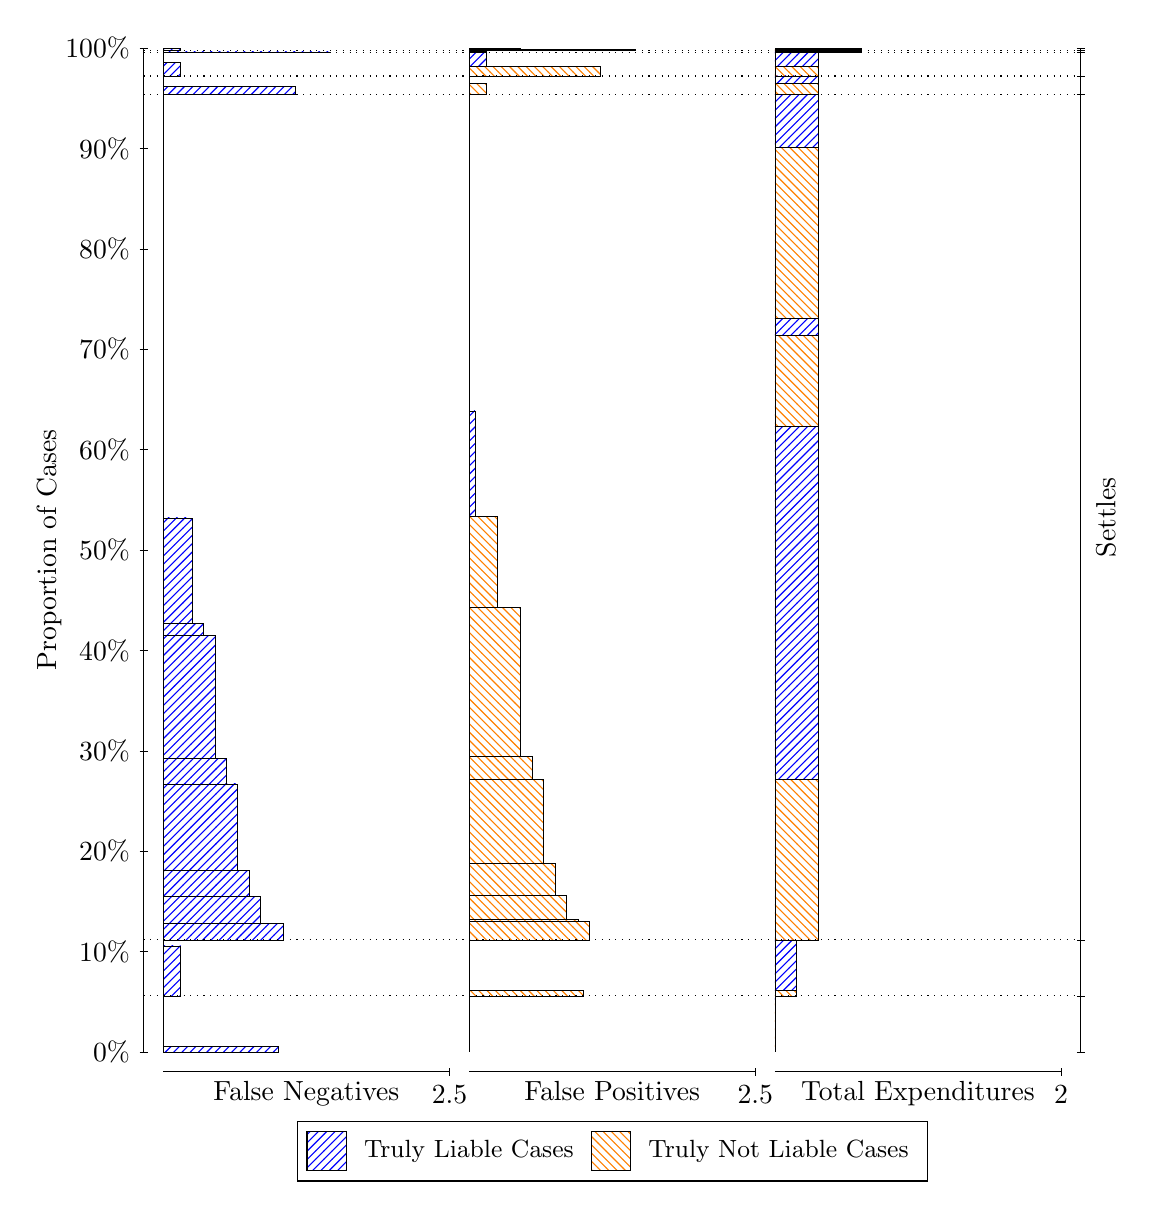
\begin{tikzpicture}
\draw[black, very thin] (1.5,1.75) -- (1.5,14.5);
\node[rotate=90, text=black, anchor=center] at (0.3, 8.125) {Proportion of Cases};
\draw[black, very thin] (1.45,1.75) -- (1.55,1.75);
\node[text=black, anchor=east] at (1.45, 1.75) {0\%};
\draw[black, very thin] (1.45,3.025) -- (1.55,3.025);
\node[text=black, anchor=east] at (1.45, 3.025) {10\%};
\draw[black, very thin] (1.45,4.3) -- (1.55,4.3);
\node[text=black, anchor=east] at (1.45, 4.3) {20\%};
\draw[black, very thin] (1.45,5.575) -- (1.55,5.575);
\node[text=black, anchor=east] at (1.45, 5.575) {30\%};
\draw[black, very thin] (1.45,6.85) -- (1.55,6.85);
\node[text=black, anchor=east] at (1.45, 6.85) {40\%};
\draw[black, very thin] (1.45,8.125) -- (1.55,8.125);
\node[text=black, anchor=east] at (1.45, 8.125) {50\%};
\draw[black, very thin] (1.45,9.4) -- (1.55,9.4);
\node[text=black, anchor=east] at (1.45, 9.4) {60\%};
\draw[black, very thin] (1.45,10.675) -- (1.55,10.675);
\node[text=black, anchor=east] at (1.45, 10.675) {70\%};
\draw[black, very thin] (1.45,11.95) -- (1.55,11.95);
\node[text=black, anchor=east] at (1.45, 11.95) {80\%};
\draw[black, very thin] (1.45,13.225) -- (1.55,13.225);
\node[text=black, anchor=east] at (1.45, 13.225) {90\%};
\draw[black, very thin] (1.45,14.5) -- (1.55,14.5);
\node[text=black, anchor=east] at (1.45, 14.5) {100\%};

\draw[black, very thin] (13.4,1.75) -- (13.4,14.5);
\draw[black, very thin] (13.35,1.75) -- (13.45,1.75);
\node[anchor=west] at (13.35, 1.75) {};
\draw[black, very thin] (13.35,2.4617) -- (13.45,2.4617);
\node[anchor=west] at (13.35, 2.4617) {};
\draw[black, very thin] (13.35,3.1734) -- (13.45,3.1734);
\node[anchor=west] at (13.35, 3.1734) {};
\draw[black, very thin] (13.35,13.911) -- (13.45,13.911);
\node[anchor=west] at (13.35, 13.911) {};
\draw[black, very thin] (13.35,14.145) -- (13.45,14.145);
\node[anchor=west] at (13.35, 14.145) {};
\draw[black, very thin] (13.35,14.443) -- (13.45,14.443);
\node[anchor=west] at (13.35, 14.443) {};
\draw[black, very thin] (13.35,14.472) -- (13.45,14.472);
\node[anchor=west] at (13.35, 14.472) {};
\draw[black, very thin] (13.35,14.5) -- (13.45,14.5);
\node[anchor=west] at (13.35, 14.5) {};

\draw[black, very thin, pattern color=blue, pattern=north east lines] (1.75,1.75) rectangle (3.2033,1.8249);
\draw[black, very thin, pattern color=orange, pattern=north west lines] (1.75,1.8249) rectangle (1.75,2.4617);
\draw[black, very thin, pattern color=blue, pattern=north east lines] (1.75,2.4617) rectangle (1.968,3.0985);
\draw[black, very thin, pattern color=orange, pattern=north west lines] (1.75,3.0985) rectangle (1.75,3.1734);
\draw[black, very thin, pattern color=blue, pattern=north east lines] (1.75,3.1734) rectangle (3.276,3.3867);
\draw[black, very thin, pattern color=blue, pattern=north east lines] (1.75,3.3867) rectangle (2.9853,3.7264);
\draw[black, very thin, pattern color=blue, pattern=north east lines] (1.75,3.7264) rectangle (2.84,4.0551);
\draw[black, very thin, pattern color=blue, pattern=north east lines] (1.75,4.0551) rectangle (2.6947,5.1547);
\draw[black, very thin, pattern color=blue, pattern=north east lines] (1.75,5.1547) rectangle (2.5493,5.4807);
\draw[black, very thin, pattern color=blue, pattern=north east lines] (1.75,5.4807) rectangle (2.404,7.0418);
\draw[black, very thin, pattern color=blue, pattern=north east lines] (1.75,7.0418) rectangle (2.2587,7.1927);
\draw[black, very thin, pattern color=blue, pattern=north east lines] (1.75,7.1927) rectangle (2.1133,8.5331);
\draw[black, very thin, pattern color=orange, pattern=north west lines] (1.75,8.5331) rectangle (1.75,13.911);
\draw[black, very thin, pattern color=blue, pattern=north east lines] (1.75,13.911) rectangle (3.4213,14.01);
\draw[black, very thin, pattern color=orange, pattern=north west lines] (1.75,14.01) rectangle (1.75,14.145);
\draw[black, very thin, pattern color=blue, pattern=north east lines] (1.75,14.145) rectangle (1.968,14.322);
\draw[black, very thin, pattern color=orange, pattern=north west lines] (1.75,14.322) rectangle (1.75,14.443);
\draw[black, very thin, pattern color=blue, pattern=north east lines] (1.75,14.443) rectangle (3.8573,14.452);
\draw[black, very thin, pattern color=orange, pattern=north west lines] (1.75,14.452) rectangle (1.75,14.472);
\draw[black, very thin, pattern color=blue, pattern=north east lines] (1.75,14.472) rectangle (1.968,14.491);
\draw[black, very thin, pattern color=orange, pattern=north west lines] (1.75,14.491) rectangle (1.75,14.5);
\draw[black, very thin, pattern color=orange, pattern=north west lines] (5.6333,1.75) rectangle (5.6333,2.3868);
\draw[black, very thin, pattern color=blue, pattern=north east lines] (5.6333,2.3868) rectangle (5.6333,2.4617);
\draw[black, very thin, pattern color=orange, pattern=north west lines] (5.6333,2.4617) rectangle (7.0867,2.5366);
\draw[black, very thin, pattern color=blue, pattern=north east lines] (5.6333,2.5366) rectangle (5.6333,3.1734);
\draw[black, very thin, pattern color=orange, pattern=north west lines] (5.6333,3.1734) rectangle (7.1593,3.4072);
\draw[black, very thin, pattern color=orange, pattern=north west lines] (5.6333,3.4072) rectangle (7.014,3.4311);
\draw[black, very thin, pattern color=orange, pattern=north west lines] (5.6333,3.4311) rectangle (6.8687,3.7344);
\draw[black, very thin, pattern color=orange, pattern=north west lines] (5.6333,3.7344) rectangle (6.7233,4.1481);
\draw[black, very thin, pattern color=orange, pattern=north west lines] (5.6333,4.1481) rectangle (6.578,5.214);
\draw[black, very thin, pattern color=orange, pattern=north west lines] (5.6333,5.214) rectangle (6.4327,5.5066);
\draw[black, very thin, pattern color=orange, pattern=north west lines] (5.6333,5.5066) rectangle (6.2873,7.3943);
\draw[black, very thin, pattern color=orange, pattern=north west lines] (5.6333,7.3943) rectangle (5.9967,8.5515);
\draw[black, very thin, pattern color=blue, pattern=north east lines] (5.6333,8.5515) rectangle (5.706,9.8919);
\draw[black, very thin, pattern color=blue, pattern=north east lines] (5.6333,9.8919) rectangle (5.6333,13.911);
\draw[black, very thin, pattern color=orange, pattern=north west lines] (5.6333,13.911) rectangle (5.8513,14.046);
\draw[black, very thin, pattern color=blue, pattern=north east lines] (5.6333,14.046) rectangle (5.6333,14.145);
\draw[black, very thin, pattern color=orange, pattern=north west lines] (5.6333,14.145) rectangle (7.3047,14.267);
\draw[black, very thin, pattern color=blue, pattern=north east lines] (5.6333,14.267) rectangle (5.8513,14.443);
\draw[black, very thin, pattern color=orange, pattern=north west lines] (5.6333,14.443) rectangle (5.8513,14.462);
\draw[black, very thin, pattern color=blue, pattern=north east lines] (5.6333,14.462) rectangle (5.6333,14.472);
\draw[black, very thin, pattern color=orange, pattern=north west lines] (5.6333,14.472) rectangle (7.7407,14.481);
\draw[black, very thin, pattern color=blue, pattern=north east lines] (5.6333,14.481) rectangle (6.2873,14.5);
\draw[black, very thin, pattern color=orange, pattern=north west lines] (9.5167,1.75) rectangle (9.5167,2.3868);
\draw[black, very thin, pattern color=blue, pattern=north east lines] (9.5167,2.3868) rectangle (9.5167,2.4617);
\draw[black, very thin, pattern color=orange, pattern=north west lines] (9.5167,2.4617) rectangle (9.7892,2.5366);
\draw[black, very thin, pattern color=blue, pattern=north east lines] (9.5167,2.5366) rectangle (9.7892,3.1734);
\draw[black, very thin, pattern color=orange, pattern=north west lines] (9.5167,3.1734) rectangle (10.062,5.214);
\draw[black, very thin, pattern color=blue, pattern=north east lines] (9.5167,5.214) rectangle (10.062,9.692);
\draw[black, very thin, pattern color=orange, pattern=north west lines] (9.5167,9.692) rectangle (10.062,10.849);
\draw[black, very thin, pattern color=blue, pattern=north east lines] (9.5167,10.849) rectangle (10.062,11.062);
\draw[black, very thin, pattern color=orange, pattern=north west lines] (9.5167,11.062) rectangle (10.062,13.243);
\draw[black, very thin, pattern color=blue, pattern=north east lines] (9.5167,13.243) rectangle (10.062,13.911);
\draw[black, very thin, pattern color=orange, pattern=north west lines] (9.5167,13.911) rectangle (10.062,14.046);
\draw[black, very thin, pattern color=blue, pattern=north east lines] (9.5167,14.046) rectangle (10.062,14.145);
\draw[black, very thin, pattern color=orange, pattern=north west lines] (9.5167,14.145) rectangle (10.062,14.267);
\draw[black, very thin, pattern color=blue, pattern=north east lines] (9.5167,14.267) rectangle (10.062,14.443);
\draw[black, very thin, pattern color=orange, pattern=north west lines] (9.5167,14.443) rectangle (10.607,14.462);
\draw[black, very thin, pattern color=blue, pattern=north east lines] (9.5167,14.462) rectangle (10.607,14.472);
\draw[black, very thin, pattern color=orange, pattern=north west lines] (9.5167,14.472) rectangle (10.607,14.481);
\draw[black, very thin, pattern color=blue, pattern=north east lines] (9.5167,14.481) rectangle (10.607,14.5);
\draw[black, dotted] (1.5,2.4617) -- (13.4,2.4617);
\draw[black, dotted] (1.5,3.1734) -- (13.4,3.1734);
\draw[black, dotted] (1.5,13.911) -- (13.4,13.911);
\draw[black, dotted] (1.5,14.145) -- (13.4,14.145);
\draw[black, dotted] (1.5,14.443) -- (13.4,14.443);
\draw[black, dotted] (1.5,14.472) -- (13.4,14.472);
\draw[black, very thin] (1.75,1.5) -- (5.3833,1.5);
\node[text=black, anchor=north] at (3.5667, 1.5) {False Negatives};
\draw[black, very thin] (5.3833,1.45) -- (5.3833,1.55);
\node[text=black, anchor=north] at (5.3833, 1.45) {2.5};

\draw[black, very thin] (5.6333,1.5) -- (9.2667,1.5);
\node[text=black, anchor=north] at (7.45, 1.5) {False Positives};
\draw[black, very thin] (9.2667,1.45) -- (9.2667,1.55);
\node[text=black, anchor=north] at (9.2667, 1.45) {2.5};

\draw[black, very thin] (9.5167,1.5) -- (13.15,1.5);
\node[text=black, anchor=north] at (11.333, 1.5) {Total Expenditures};
\draw[black, very thin] (13.15,1.45) -- (13.15,1.55);
\node[text=black, anchor=north] at (13.15, 1.45) {2};



\node[text=black, centered, rotate=90] at (13.72, 8.5423) {Settles};





\draw (7.449999999999999,1.5) node[draw=none] (baseCoordinate) {};
\begin{scope}[align=center]
        \matrix[scale=0.5, draw=black, below=0.5cm of baseCoordinate, nodes={draw}, column sep=0.1cm]{
            \node[rectangle, draw, minimum width=0.5cm, minimum height=0.5cm, pattern color=blue, pattern=north east lines] {}; &
            \node[draw=none, font=\small, text=black] (B) {Truly Liable Cases}; &
            \node[rectangle, draw, minimum width=0.5cm, minimum height=0.5cm, pattern color=orange, pattern=north west lines] {}; &
            \node[draw=none, font=\small, text=black] (B) {Truly Not Liable Cases}; \\
            };
\end{scope}

\end{tikzpicture}
\end{document}